\documentclass[a4paper,10pt]{article}

\usepackage[utf8]{inputenc}
\usepackage[T1]{fontenc}
\usepackage{float}
\usepackage{tikz}
\usepackage{tikz-uml} 
\usepackage{amsmath}


% custom listing settings
\usepackage{listings}
\usepackage{lstcustom}
\usepackage[utf8]{inputenc}
\usepackage[T1]{fontenc}
\usepackage[scaled=0.8]{beramono} % beramono or luximono give very nice ttfamily fonts
\renewcommand{\lstfontfamily}{\ttfamily}

\newcommand{\reffig}[1]{figure \ref{fig:#1}}

%\usepackage{minted}


%\maketitle

%\begin{abstract}
%This document describes the general architecture of the BornAgain project.
%\end{abstract}


\title{BornAgain. }
\author{}



\begin{document}
A software to simulate and fit neutron and x-ray scattering at grazing incidence
Some software


%%%%%%%%%%%%%%%%%%%%%%%%%%%%%%%%%%%%%%%%%%%%%%%%%%%%%%%%%%%%%%%%%%%%%%%%%%%%%%%%
%%
%%   BornAgain User Manual
%%
%%   homepage:   http://www.bornagainproject.org
%%
%%   copyright:  Forschungszentrum Jülich GmbH 2015
%%
%%   license:    Creative Commons CC-BY-SA
%%
%%   authors:    Scientific Computing Group at MLZ Garching
%%               C. Durniak, M. Ganeva, G. Pospelov, W. Van Herck, J. Wuttke
%%
%%%%%%%%%%%%%%%%%%%%%%%%%%%%%%%%%%%%%%%%%%%%%%%%%%%%%%%%%%%%%%%%%%%%%%%%%%%%%%%%


\cleardoublepage
\ichapter{Introduction}

%%%%%%%%%%%%%%%%%%%%%%%%%%%%%%%%%%%%%%%%%%%%%%%%%%%%%%%%%%%%%%%%%%%%%%%%%%%%%%%%
\isection{About BornAgain}
%%%%%%%%%%%%%%%%%%%%%%%%%%%%%%%%%%%%%%%%%%%%%%%%%%%%%%%%%%%%%%%%%%%%%%%%%%%%%%%%

\BornAgain\ is a software package
to simulate and fit
reflectometry, off-specular scattering,
and grazing-incidence small-angle scattering (GISAS)
of X-rays and neutrons.
It provides a generic framework
for modeling multilayer samples with smooth or
rough interfaces and with various types of embedded nanoparticles.
Support for neutron polarization and magnetic scattering
is under development.
The name, \BornAgain,
alludes to the central role of the distorted-wave Born
approximation (DWBA) in the physical description of the
scattering process.
\index{Distorted-wave Born approximation}

\BornAgain\ is being developed
by the Scientific Computing Group
of the J\"ulich Centre for Neutron Science (JCNS)
at Heinz Maier-Leibnitz Zentrum (MLZ) Garching, Germany.
It is intended to serve experimentalists in analysing all kinds
of reflectometry data.
It is equally aimed at users of MLZ reflectometers
\cite{mlz:maria,mlz:nrex,mlz:refsans},
at JCNS in-house researchers,
and at the reflectometry and GISAS community at large.
It is the main contribution of JCNS to national \cite{ba:hdri}
and international \cite{ba:sine2020} collaborations
of large-scale facilities for the development of better user software.

\BornAgain\ is released as free and open source software under
the GNU General Public License (GPL, version 3 or higher).
This documentation comes under the Creative Commons license CC-BY-SA.

\Warn{\indent The converse of this liberal policy is
that we cannot guarantee correctness and accuracy of the code.
It is entirely in the responsibility of users
to convince themselves that their data interpretation
is physically meaningful and plausible.}
\Work{\indent\BornAgain\ is still under intense development.
New major versions are released about every few months.
When need arises, bugfix versions are released in between.
It is strongly recommended that users regularly update their installations.}

The software \BornAgain\ embodies nontrivial scientific ideas.
Therefore when \BornAgain\ is used in preparing scientific papers,
it is mandatory to cite the software:
\index{Citation}%
%\marginpar{citation}%
\begin{quote}
\authors\ (2013--\the\year),\newline
BornAgain --- Software for simulating and fitting
X-ray and neutron small-angle scattering at grazing incidence,
version [\ldots],\newline
\url{http://www.bornagainproject.org}
\end{quote}
The initial design of \BornAgain\ owes much
to the widely used program \IsGISAXS\
\index{IsGISAXS@\IsGISAXS}%
\index{Lazzari, R\'emi}%
by R\'emi Lazzari \cite{Laz02,Laz08}.
Therefore when using \BornAgain\ in scientific work,
it might be appropriate to also cite the pioneering papers
by Lazzari \etal\ \cite{Laz02,ReLL09}.

Since version 1.0, \BornAgain\
almost completely reproduces the functionality
of \IsGISAXS.
About 20 exemplary simulations have been tested against \IsGISAXS,
and found to agree up to almost the last floating-point digit.
\BornAgain\ goes beyond \IsGISAXS\
in supporting an unrestricted number of layers and particles,
diffuse reflection from rough layer interfaces and
particles with inner structures.
Support for neutron polarization and magnetic scattering
is under development.
Adhering to a strict object-oriented design,
\BornAgain\ provides a solid base for future extensions
in response to specific user needs.

%%%%%%%%%%%%%%%%%%%%%%%%%%%%%%%%%%%%%%%%%%%%%%%%%%%%%%%%%%%%%%%%%%%%%%%%%%%%%%%%
\isection{Registration, contact, discussion forum}\label{Snews}
%%%%%%%%%%%%%%%%%%%%%%%%%%%%%%%%%%%%%%%%%%%%%%%%%%%%%%%%%%%%%%%%%%%%%%%%%%%%%%%%

\index{Registration}
\index{Newsletter}
To stay informed about the ongoing development of \BornAgain,
register on the project homepage \url{http://www.bornagainproject.org}
(``Create new account'').
You will then receive our occasional newsletters,
and be authorized to post to the discussion forum.

\index{Contact}
To contact the \BornAgain\ development and maintenance team
in the Scientific Computing Group
of Heinz Maier-Leibnitz Zentrum (MLZ) Garching,
write a mail to \url{contact@bornagainproject.org},
or fill the form in the \textsc{Contact} section of the
project web site.

\index{Forum}
For questions that might be of wider interest,
please consider posting to the discussion forum,
accessible through the \textsc{Forums} tab of the project web site.

\index{Bug reports}%
Please contact us for any question not answered here
or in the online documentation.
We are grateful for all kind of feedback:
criticism, praise, bug reports, feature requests or contributed modules.
If questions go beyond normal user support,
we will be glad to discuss a scientific collaboration.

%%%%%%%%%%%%%%%%%%%%%%%%%%%%%%%%%%%%%%%%%%%%%%%%%%%%%%%%%%%%%%%%%%%%%%%%%%%%%%%%
\isection{About this Manual}
%%%%%%%%%%%%%%%%%%%%%%%%%%%%%%%%%%%%%%%%%%%%%%%%%%%%%%%%%%%%%%%%%%%%%%%%%%%%%%%%

This User Manual is complementary to the online documentation
at \url{http://www.bornagainproject.org}.
It does not duplicate information that is more conveniently read online.
The online documentation covers in particular
how to download and install \BornAgain.

This User Manual containes of two parts:
\Cref{PPHYS} provides physics background
on the scattering theory and on the sample models implemented in \BornAgain.
\cref{PREF} is a partial reference of the C$++$ and Python interfaces;
it concentrates on physics related component,
and thereby complements the automatically generated interface documentation
that can be found online at \url{http://apps.jcns.fz-juelich.de/doxy/BornAgain/index.html}.

\Work{\indent This manual is incomplete.
Several important chapters are still incomplete, or only consist of a placeholder.}
We intend to publish the missing material successively,
along with new software release.

\pagebreak[3]
We use the following colored boxes to highlight
certain information:

\def\demobox#1{\noindent\strut\hspace{.2\TW}\begin{minipage}{.75\textwidth}#1
\end{minipage}\hfill\strut}

\medskip
\demobox{\Warn{\indent Such a box contains
a \textbf{warning} about potential problems
with the software or the documentation.}}

\medskip
\demobox{\Work{\indent This road sign in the margin indicates \textbf{work in progress}.}}

\medskip
\demobox{\Emph{\indent A green box highlights
  an \textbf{important fact}, for instance an equation
  that is central in
  the further development of the theory.}}

\medskip
\demobox{\Note{\indent
  An \textbf{implementation note} explains
  how the theory exposed in this manual is actually used in \BornAgain.}}

\medskip
\noindent\strut\hspace{.2\TW}This is a \tuto{1}{link to the online docs}.

\medskip
\setCpp
\begin{lstlisting}[linewidth=.95\TW,xleftmargin=.2\TW]
C++ code, mainly used for API documentation.
\end{lstlisting}

\setPy
\begin{lstlisting}[linewidth=.95\TW,xleftmargin=.2\TW]
Python code.
\end{lstlisting}

\bigskip
Mathematical notations are explained in the symbol index, page~\pageref{Snomencl}.

\newpage
\section{Installation} \SecLabel{installation}

This section shortly describes how to build \BornAgain\ from source and run first
simulation.

\documentclass[a4paper,10pt]{article}
\usepackage[utf8]{inputenc}
\usepackage[T1]{fontenc}
\usepackage{tikz}
\usepackage{tikz-uml} 
\usepackage{amsmath}


%opening
\title{}
\author{}

\begin{document}

%\maketitle

%\begin{abstract}
%\end{abstract}

%\section{}

\begin{tikzpicture}
\begin{umlpackage}{Sample description} 
% Code from official documentation goes here...
\umlinterface{ISample}{
}{
  \umlvirt{+ clone() : ISample*} \\
  \umlvirt{+ createDWBASimulation() : DWBASimulation*}
}
\umlclass[y=-4]{MultiLayer}{
  -- m\_layers : std::vector<Layer *> \\
  -- m\_interfaces : std::vector<LayerInterface *>
}{
  + getNumberOfLayers() : size\_t \\
  + getNumberOfInterfaces() : size\_t \\
  + addLayer(const Layer \&layer) : void
}
\umlclass[x=8,y=-4]{Layer}{
  -- mp\_material : IMaterial* \\
  -- m\_thickness : double
}{
  + getThickness() : double \\
  + setThickness(double thickness) : void
}
\umlinherit[geometry=-|]{MultiLayer}{ISample}
\umlinherit[geometry=|-]{Layer}{ISample}
\umluniassoc[geometry=--, mult2=n]{MultiLayer}{Layer}
\end{umlpackage}
\end{tikzpicture}

\begin{tikzpicture}
\begin{umlpackage}{Simulation Data}
\umlclass{Experiment}{
  -- mp\_sample : ISample* \\
  -- mp\_sample\_builder : ISampleBuilder* \\
  -- m\_detector : Detector \\
  -- m\_beam : Beam \\
  -- m\_intensity\_map : OutputData<double> \\
  -- m\_sim\_params : SimulationParameters
}{
  \umlvirt{+ clone() : Experiment*} \\
  \umlvirt{+ runSimulation() : void} \\
  \umlvirt{+ normalize() : void}
}
\umlemptyclass[x=7, y=0]{ISample}
\umlemptyclass[x=7, y=-2]{Detector}
\umlemptyclass[x=7, y=-4]{Beam}
\umlemptyclass[x=7, y=-6]{SimulationParameters}
\umlemptyclass[y=-4]{GISASExperiment}
\umluniassoc[geometry=|-, anchor1=0]{Experiment}{ISample}
\umluniassoc[geometry=|-, anchor1=0]{Experiment}{Detector}
\umluniassoc[geometry=|-, anchor1=0]{Experiment}{Beam}
\umluniassoc[geometry=|-, anchor1=0]{Experiment}{SimulationParameters}
\umlinherit[geometry=--]{GISASExperiment}{Experiment}

\umlnote[y=-6.5, width=6cm]{GISASExperiment}{
  The ``runSimulation()'' method retrieves an ISimulation object
  from the topmost ISample object and calls its ``run()'' method 
  to perform the actual computations.
}
  
\end{umlpackage}


\end{tikzpicture}

\end{document}

\newpage
\chapter{Fitting}

%     Minuit Library:
%         Migrad Algorithm ("Minuit", "Migrad"),
%         Simplex Algorithm ("Minuit", "Simplex")
%         Minimize Algorithm ("Minuit", "Minimize")
%         Scan Algorithm ("Minuit", "Scan")
%         Seek Algorithm ("Minuit", "Seek")
%     Fumili Library:
%         Fumili Algorithm
%     Minuit2 Library:
%         Migrad Algorithm ("Minuit2", "Migrad")
%         Simplex Algorithm ("Minuit2", "Simplex")
%         Minimize Algorithm ("Minuit2", "Minimize")
%         Scan Algorithm ("Minuit2", "Scan")
%         Fumili2 Algorithm ("Minuit2", "Fumili2")
%     GSL Library: (Only available if GSL and MathMore are avaiable too)
%         Fletcher-Reeves Conjugate Gradient Algorithm ("GSLMultiMin", "conjugatefr")
%         Polak-Ribiere Conjugate Gradient Algorithm ("GSLMultiMin", "conjugatepr")
%         BFGS Conjugate Gradient Algorithm ("GSLMultiMin", "bfgs2")
%         Levenberg-Marquardt Algorithm ("GSLMultiFit", "")
%         Simulated Annealing Algorithm ("GSLSimAn", "")

In addition to the simulation of grazing incidence
x-ray and neutron scattering by
multilayered samples, BornAgain also offers the option to
fit a selection of simulated sample parameters to experimental data.  This aspect
of the software is discussed in this chapter.

%%%%%%%%%%%%%%%%%%%%%%%%%%%%%%%%%%%%%%%%%%%%%%%%%%%%%%
\section{Short description of fitting theory}

These features of BornAgain deal with estimating the optimum parameters
in the simulation by minimizing the difference ($\chi^2$) between theory and experimental data.\\

\textbf{From Minuit user's guide}: Minuit is usually used to find the ``best'' values of a set of
parameters, where ``best'' is defined as those values which minimize a
given function, FCN. The width of the function minimum in some
neighbourhood of the minimum, gives information about the uncertainty
in the best parameter values. An important feature of Minuit is that
it offers several tools to analyze the parameter errors.



\noindent \smallpencil \colorbox{Lightgray}{\parbox{\dimexpr\linewidth-8\fboxsep}
{\underline{Theory}: Users wanting to find out more about minimization (also called
maximization or optimization methods) are referred to \ldots.}}\\

%The conjugate gradient and BFGS methods are described in detail in the following book,
%    R. Fletcher, Practical Methods of Optimization (Second Edition) Wiley (1987), ISBN 0471915475. 
%A brief description of multidimensional minimization algorithms and more recent references can be found in,
%    C.W. Ueberhuber, Numerical Computation (Volume 2), Chapter 14, Section 4.4 Minimization Methods, p. 325–335, Springer (1997), ISBN 3-540-62057-5
%The simplex algorithm is described in the following paper,
%    J.A. Nelder and R. Mead, A simplex method for function minimization, Computer Journal vol. 7 (1965), 308–313. 
% W. T. Eadie, D. Drijard, F. James, M. Roos, and B. Sadouletm
% Statistical methods in experimental physics, North-Holland 1971

Local minimum, multiple minima

%\url{http://seal.web.cern.ch/seal/MathLibs/Minuit2/html/}

%\url{http://seal.web.cern.ch/seal/documents/minuit/mntutorial.pdf}

%\url{http://root.cern.ch/root/html/MATH_MINUIT2_Index.html}

A detailed tutorial of Minuit software can be downloaded at the
following address \url{http://seal.web.cern.ch/seal/documents/minuit/mnusersguide.pdf}.
%\cite{MinuitRoot}.

Local or global minimization
%%%%%%%%%%%%%%%%%%%%%%%%%%%%%%%%%%%%%%%%%%%%%%%%%%%%%%
\section{Implementation in BornAgain}
BornAgain fitting features include...\\
Different geometries, number of fit parameters, variety of minimizers\\
and minimization strategies.\\

Minimizer belongs to MinimizerFactory (interacts with Root)

Variable parameters: customize lists, inputs required, default values

Methods: implemented list, possibility to add your own.

Set/create minimizer : name + algorithm + option (part of Minimizer
factory). The minimizers can be chosen from the following list:

FitSuite: m\_minimizer, m\_is\_last\_iteration

\textbf{Questions}
\begin{itemize}
\item Is it possible to fit on the particle kind (cylinder or prism or
\ldots)?
\item Fit using several experimental runs?
\item Number of degrees of freedom?
\item Weighted fits?
\item Errorbars, epsilon for standard error
\item Normalisation of the data (in order to be compared)
\item Constraints between parameters
\item Quick fit option
\item Possible exponential decrease of the form factor
\item fit of 1D plots?
\end{itemize}
%To run tests: python TestFit.py\\
%List of tests\\
%TestFit01 - Two parameter fit using variety of minimizers. Geometry: cylinders in the air.\\
%TestFit02 - Fitting using sample builder\\


Class TestFittingModule1: 
\begin{itemize}
\item mp\_real\_data (experimental data), 
\item mp\_simulated\_data,
\item mp\_simulation, 
\item mp\_sample, 
\item mp\_fitsuite: \texttt{addSimulationAndRealdData}: link a given set of experimental data with a
  particular set of simulated data in order to proceed to a fit. It is
  therefore possible to generate a batch of different numerical
  samples to test different configurations in order to obtain the best
  fit by playing with the number of layers or the shape of particles
  (different form factors). What about \texttt{chi2\_module} by default?
\end{itemize} 

\texttt{attachObserver} uses
\texttt{FitSuiteObserverFactory::CreatePrintObserver()} or
\texttt{FitSuiteObserverFactory::CreateDrawObserver()} or
\texttt{FitSuiteObserverFactory::CreateTreeObserver()}.


%runFit()

%%%%%%%%%%%%%%%%%%%%%%%%%%%%%%%%%%%%%%%
\subsubsection{General procedure to fit / for fitting}

Format of input (experimental data) - requirements (structure,
normalisation, values...)
Experimental data can be entered by importing it from ASCII files created by other applications.
%Therefore the number of layers cannot be used as a fitting parameter

A fit is run for a fixed value of \textbf{the number of layers
  constituting the sample}, the \textbf{input beam wavelength}.

Input = matrix of intensity as function of ?

Generation of the numerical model (cf other examples or detailed
description or only script given and description of main steps)

\textbf{Structure of fitting module in BornAgain.}


\textbf{Structure of Fit folder (sources *.cpp):}
\begin{itemize}
\item FitObject.cpp
\item FitSuiteObjects.cpp		
\item MinimizerFactory.cpp
\item ROOTMinimizer.cpp
\item FitParameter.cpp		
\item FitSuiteParameters.cpp		
\item MinimizerScan.cpp		
\item ROOTMinimizerHelper.cpp
\item FitParameterLinked.cpp		
\item FitSuitePrintObserver.cpp	
\item MinimizerTest.cpp
\item FitSuite.cpp			
\item FitSuiteStrategies.cpp		
\item ROOTGSLNLSMinimizer.cpp
\item FitSuiteFunctions.cpp		
\item IFitSuiteStrategy.cpp
\item ROOTGSLSimAnMinimizer.cpp
\end{itemize}

\textbf{Structure of Fit folder (headers *.h):}
\begin{itemize}
\item AttFitting.h		
\item FitSuite.h		
\item FitSuiteStrategies.h	
\item MinimizerTest.h		
\item ROOTMinimizerHelper.h
\item AttLimits.h		
\item FitSuiteFunctions.h	
\item IFitSuiteStrategy.h	
\item ROOTGSLNLSMinimizer.h
\item FitObject.h		
\item FitSuiteObjects.h	
\item IMinimizer.h		
\item ROOTGSLSimAnMinimizer.h
\item FitParameter.h		
\item FitSuiteParameters.h	
\item MinimizerFactory.h	
\item ROOTMinimizer.h
\item FitParameterLinked.h	
\item FitSuitePrintObserver.h	
\item MinimizerScan.h		
\item ROOTMinimizerFunction.h
\end{itemize}

\myparagraph{\underline{Choice of parameters to be fitted}}
In principle, every parameter used in the construction of the sample
can be used as a fit parameter. For example

\begin{table}[h]
\centering
\begin{tabular}{|@{}l||l@{}|}
\hline
\textbf{Particles} &  dimensions: height, radius, length, width, \\
                             &  half side length, thickness, \textbf{index of refraction} 
                             height\_aspect\_ratio, \textbf{orientation?} \\
& (depending on the shape) \\
& inteference (density, proportion, width, distance,\\
& probability,
dispersion radius) \\
\hline
\textbf{Lattice} & \\
\hline
\textbf{Layers} & roughness, thickness, \textbf{index of refraction} \\
\hline
\textbf{Beam} & intensity \\
\hline
\textbf{Detector} & \\
\hline
\end{tabular}
\label{table:fitting_parameters}
\caption{List of parameters that can be defined as fitting parameters.}
\end{table}

The heights of different particles can be associated to two different
fitting parameters and optimized / minimized separately.


m\_cylinder\_ratio, m\_cylinder\_height
m\_prism3\_half\_side, m\_prism3\_height
                          
  *Normalizer/scale
  *Normalizer/shift

  *SampleBuilder/particle\_probability1
  *SampleBuilder/particle\_radius1
  *SampleBuilder/dispersion\_radius1
  *SampleBuilder/height\_aspect\_ratio1

  *SampleBuilder/interf\_distance
  *SampleBuilder/interf\_width

 *SampleBuilder/height\_aspect\_ratio
 
   */lattice\_length\_a 
   */lattice\_length\_c   
   */nanoparticle\_radius",     
   */sigma\_nanoparticle\_radius
   */meso\_height       
   */meso\_radius  
   */sigma\_meso\_height
   */sigma\_meso\_radius
   */sigma\_lattice\_length\_a
   */surface\_filling\_ratio
   */roughness

 
In BornAgain, the parameters used for the fit are specified using the
function \texttt{addFitParameter} with the following syntax:

\begin{lstlisting}[language=C++, style=eclipse,numbers=none]
m\_fitSuite->addFitParameter("*height", 4.*Units::nanometer,
0.04*Units::nanometer, AttLimits::lowerLimited(0.01) );

m\_fitSuite->addFitParameter("*radius", 6.*Units::nanometer,
0.06*Units::nanometer, AttLimits::lowerLimited(0.01) );

m\_fitSuite->addFitParameter("*SampleBuilder/m\_cylinder\_height",4*Units::nanometer, 0.01*Units::nanometer,AttLimits::lowerLimited(0.01) );

m\_fitSuite->addFitParameter("*SampleBuilder/m\_cylinder\_radius",
  6*Units::nanometer, 0.01*Units::nanometer, AttLimits::lowerLimited(0.01) );

m\_fitSuite->addFitParameter("*SampleBuilder/m\_prism3\_half\_side", 4*Units::nanometer, 0.01*Units::nanometer,  AttLimits::lowerLimited(0.01) );
\end{lstlisting}

There are two possible syntaxes:
\begin{itemize}
\item First option: \\ \texttt{m\_fitSuite->addFitParameter(name, value, step, attlim, error);},
where \texttt{value}, \texttt{step} and \texttt{error} are double values corresponding to the ... respectively.
\item Second option: \\
\texttt{m\_fitSuite->addFitParameter(name, value, attlim, error);}
\end{itemize}

\texttt{attlim} is , \texttt{name} is ...
By default the input value of \texttt{error} is 0.
 

\texttt{AttLimits} can be
\begin{itemize}
\item fixed(), 
\item lowerLimited(double value), 
\item limited(double min value, double max value).
\end{itemize}
The unit of \texttt{AttLimits} is  identical to the one used to characterize the
parameter.

Number of iterations
Interrupt fit
Procedure: initially choose a small number of fitting parameters

\textbf{ Software Scatter :The program allows to automatically fit large number of data files such as files from timeresolved
studies. A requirement is that subsequent scattering curves do not differ too much, so
that the fitted values of the first curve can be used as starting parameters for a fit to the next
curve. Before starting a fit series, choose the first data file and perform a fit so that the
parameter values are set to an optimal start value. The first/last point, qmin/max and Imin for
the fit will apply to all data sets.}

Background noise, intensity threshold.


%%%%%%%%%%%%%%%%%%%%%%%%%%%%%%%%%%%%%%%
\subsubsection{Fitting methods implemented}

\textbf{Is there any default method implemented?}
Different minimizers from Root library can be used in BornAgain. They are listed in
Table~\ref{table:fit_minimizers}. Users can also add their own by
implementing their definition in the \texttt{Catalogue} contained in
program \texttt{MinimizerFactory}.
Minuit user's manual describes which minimizer to use in order to best
fit our data\ldots  \cite{MinuitRoot}.

\begin{table}[h]
\centering
\begin{tabular}{@{}ll@{}}
\hline
\hline
\textbf{Minimizer name - Library} & \textbf{Algorithm} \\
\hline
%Test & \\
%Scan & \\%[-3pt] 
Minuit & Migrad, Simplex, Combined, Scan\\
Minuit2 & Migrad, Simplex, Combined, Scan, Fumili \\
Fumili & \\
GSLMultiMin & ConjugateFR, ConjugatePR, BFGS, BFGS2, SteepestDescent \\
GSLMultiFit & \\
GSLSimAn & \\ %Simulatded annealing algorithm
Genetic &  \\ %TMVA Toolkit for Multivariate Data Analysis with ROOT 
\hline
\hline
\end{tabular}
\label{table:fit_minimizers}
\caption{List of fitting minimizers implemented in BornAgain.}
\end{table}




Minuit2, originally developed in the SEAL project, is now distributed
within ROOT. The classes have been moved inside the namespace
ROOT::Minuit2. 

Minuit is conceived as a tool to find the minumum value of a
multi-parameter function and analyze the shape of the function around
the minimum. The principal application is foreseen for statistical
analysis, working on chisquare or log-likelihood functions, to compute
the best-fit parameter values and uncertainties, including
correlations between the parameters. It is especially suite to handle
difficult problems, including those which may requier guidance in
order to find the correct solution.

Minuit2, optional package in the ROOT framework, is a numerical minimization computer program
originally written in C++ programming language. The program searches for minima in a user-defined function with
respect to one or more parameters using several different methods as
specified by the user. 
%%%%%%%%%%%%%%%%%%%%%%%%%%%%%%%%%%%%%%%
\subsubsection{Outputs}
log file, how to interpret the data, how to save the estimated parameters.
Customize using \texttt{Observer}.
See FitGISAXS, IsGISAXS, Fish.
%%%%%%%%%%%%%%%%%%%%%%%%%%%%%%%%%%%%%%%%%%%%%%%%%%%%%%
\section{Examples}
in C++ or Python?
TestPyFit: testfit01.py, testfit02.py
FitSuite

Observer

Screenshot after running the program
Graph?
Simulation
Real data


Difference between TestFit and TestPyFit

Different steps to follow - order of execution

%%%%%%%%%%%%%%%%%%%%%
\myparagraph{\underline{First step:} Initializing the simulation}

 definition of the detector's
  parameters \texttt{setDetectorParameters} and the beam's parameters
  \texttt{setBeamParameters}

%%%%%%%%%%%%%%%%%%%%%
\myparagraph{\underline{Generating the sample}}

Layers, particles, 

%%%%%%%%%%%%%%%%%%%%%
\myparagraph{\underline{Choice of parameters to be fitted}}

choice of parameters
  to be used for minimization \texttt{addFitParameter}. 

%%%%%%%%%%%%%%%%%%%%%
\myparagraph{\underline{Running the simulation / the fit}}

Normalisation ?

Output = two-dimensional matrix.

How to run the fit: using the function \texttt{fit}



\begin{lstlisting}[caption={Python script of fitting example},
  label=script_exfit1,captionpos=b,escapeinside={@}{@} ,language=python,style=eclipse, numbers= none,frame = leftline ,
      framerule = 2mm ,
      rulecolor = \color{lightgrey},
      breaklines = true]
# In this test we are using simple geometry: cylinders without interference in
# air layer with two parameters (radius and height of cylinders), describing
# the sample. Our "real" data is 2D intensity map obtained from the simulation of
# the same geometry with fixed values height = 5nm and radius = 5nm.
# Then we run our minimization consequently using different minimization engines,
# with height=4nm, radius=6nm as starting fit parameter values.
import sys
import os
import numpy
import time

sys.path.append(os.path.abspath(
                os.path.join(os.path.split(__file__)[0],
                '..', '..', '..', 'lib')))

from libBornAgainCore import *
from libBornAgainFit import *

# sample parameters we are going to find
cylinder_height = 5*nanometer
cylinder_radius = 5*nanometer

# minimizer name and type of minimization algorithm
Minimizers = [ 
    ("Minuit2","Migrad"), 
    ("Minuit2","Fumili"), 
    ("GSLMultiMin","BFGS"),
    ("GSLMultiMin","SteepestDescent"),
    ("GSLMultiFit",""),
#    ("GSLSimAn","")
]

# -----------------------------------------------------------------------------
# run several minimization rounds using different minimizers
# -----------------------------------------------------------------------------
def runTest():
    #print "**********************************************************************"
    #print "*  Starting  TestFit01                                               *"
    #print "**********************************************************************"
    nTest=0
    status = "OK"
    for m in Minimizers:
        minimizer_name = m[0]
        minimizer_algorithm = m[1]
        print "Minimizer {0:-2d}   {1:}({2:})".format(nTest, minimizer_name, minimizer_algorithm)
        result_ok = run_fitting(minimizer_name, minimizer_algorithm)
        nTest+=1
        if not result_ok: status = "FAILED"

    return "TestFit01", "Two parameters fit using variety of minimizers.", status

# -----------------------------------------------------------------------------
# run fitting specified minimizer
# -----------------------------------------------------------------------------
def run_fitting(minimizer_name, minimizer_algorithm):
    sample = buildSample()
    simulation = createSimulation()
    simulation.setSample(sample)

    # creating real data, which is simply results of our simulation with default values
    simulation.runSimulation()
    real_data = simulation.getOutputDataClone()

    # setting fit suite
    fitSuite = FitSuite()
    fitSuite.setMinimizer( MinimizerFactory.createMinimizer(minimizer_name, minimizer_algorithm) )
    fitSuite.addFitParameter("*height", 4.*nanometer, 0.04*nanometer, AttLimits.lowerLimited(0.01) )
    fitSuite.addFitParameter("*radius", 6.*nanometer, 0.06*nanometer, AttLimits.lowerLimited(0.01) )
    fitSuite.addSimulationAndRealData(simulation, real_data)

    # run fit
    start_time = time.time()
    fitSuite.runFit()
    real_time = time.time() - start_time

    height_found = fitSuite.getMinimizer().getValueOfVariableAtMinimum(0)
    height_diff = abs(height_found - cylinder_height)/cylinder_height
    radius_found = fitSuite.getMinimizer().getValueOfVariableAtMinimum(1)
    radius_diff = abs(radius_found - cylinder_radius)/cylinder_radius

    print "            RealTime : {0:.3f} sec".format(real_time)
    print "            NCalls   : {0:<5d}".format(fitSuite.getNCalls())
    print '            par1     : {0:.4f} ({1:.3g}) '.format(height_found, height_diff)
    print '            par2     : {0:.4f} ({1:.3g}) '.format(radius_found, radius_diff)

    diff = 1.0e-02
    isSuccess = True
    if( (height_diff > diff) or (radius_diff > diff) ) : isSuccess=False
    return isSuccess

# -----------------------------------------------------------------------------
# create cylinders in the air
# -----------------------------------------------------------------------------
def buildSample():
    cylinder_ff = FormFactorCylinder(cylinder_height, cylinder_radius)
    n_particle = complex(1.0-6e-4, 2e-8)
    cylinder = Particle(n_particle, cylinder_ff)
    interference = InterferenceFunctionNone()

    particle_decoration = ParticleDecoration()
    particle_decoration.addParticle(cylinder)
    particle_decoration.addInterferenceFunction(interference)

    mAmbience = MaterialManager.getHomogeneousMaterial("Air", 1.0, 0.0 )
    air_layer = Layer(mAmbience)
    air_layer_decorator = LayerDecorator(air_layer, particle_decoration)
    multi_layer = MultiLayer()
    multi_layer.addLayer(air_layer_decorator)

    return multi_layer

def createSimulation():
    simulation = Simulation();
    simulation.setDetectorParameters(100, 0.0*degree, 2.0*degree,100 , 0.0*degree, 2.0*degree);
    simulation.setBeamParameters(1.0*angstrom, -0.2*degree, 0.0*degree);
    simulation.setBeamIntensity(1e10);
    return simulation

#-------------------------------------------------------------
# main()
#-------------------------------------------------------------
if __name__ == '__main__':
    name,description,status = runTest()
    print name,description,status
    if("FAILED" in status) : exit(1)
\end{lstlisting}


Output of functional test: fit module 2 params

TestFittingModule1.cpp with "Minuit2", "Migrad"

\begin{lstlisting}[style=eclipse,numbers=none]
FitSuitePrintObserver::update() -> Info. NCall:0 NStrategy:0 Chi2:6.26500281e+09
Time spend since last call, cpu:0.03 sec, wall time 0.03sec
   # 0 *height                                 4.00000000e+00  lim(0.01,)
   # 1 *radius                                 6.00000000e+00  lim(0.01,)
FitSuitePrintObserver::update() -> Info. NCall:20 NStrategy:0 Chi2:9.29429839e+07
Time spend since last call, cpu:1.27 sec, wall time 4.72sec
   # 0 *height                                 4.51488966e+00  lim(0.01,)
   # 1 *radius                                 4.68705140e+00  lim(0.01,)
FitSuitePrintObserver::update() -> Info. NCall:40 NStrategy:0 Chi2:9.74308159e+05
Time spend since last call, cpu:0.97 sec, wall time 1.05sec
   # 0 *height                                 4.94285364e+00  lim(0.01,)
   # 1 *radius                                 5.07666127e+00  lim(0.01,)
FitSuitePrintObserver::update() -> Info. NCall:60 NStrategy:0 Chi2:7.91181985e+00
Time spend since last call, cpu:1.00 sec, wall time 1.07sec
   # 0 *height                                 4.99977322e+00  lim(0.01,)
   # 1 *radius                                 4.99985065e+00  lim(0.01,)
FitSuitePrintObserver::update() -> Info. NCall:80 NStrategy:0 Chi2:1.01820395e-02
Time spend since last call, cpu:0.98 sec, wall time 1.05sec
   # 0 *height                                 5.00000020e+00  lim(0.01,)
   # 1 *radius                                 5.00000004e+00  lim(0.01,)

FitSuiteObserverPrint::update() -> Info. Printing results

--- FitSuite::printResults --------------------------
 Chi2:1.19798858e-02    chi2.NCall:85  grad.NCall:0,0,0 (neval, ngrad, total)
   # 0 *height                                 4.99999992e+00  lim(0.01,)
   # 1 *radius                                 5.00000004e+00  lim(0.01,)
-----------------------------------------------------
  MinimizerType          : Minuit2
  MinimizerAlgorithm     : Migrad
--- Options -----------------------------------------
  Strategy               : 1
  Tolerance              : 0.01
  MaxFunctionCalls       : 10000
  MaxIterations          : 10000
  Precision              : -1.00
  ErrorDefinition        : 1.00 (1-chi2, 0.5 likelihood)
  ExtraOptions           : 0
--- Status ------------------------------------------ 
  Status                 : 0 'OK, valid minimum'
  IsValidError           : 0 'No detailed error validation'
  CovMatrixStatus        : 3 'full accurate'
  NCalls                 : 85
  MinValue               : 1.01756899e-02
  Edm                    : 4.39332982e-12
--- Variables ---------------------------------------
  NumberOfVariables      : 2 (free), 2 (total) 
  Errors                 : yes, see below
      Npar  Name                                  Value         Error         GlobalCC      
      0    *height                                5.000000e+00  1.109913e-04  1.208255e-01  
      1    *radius                                5.000000e+00  8.941040e-05  1.208255e-01  
--- Correlations-------------------------------------
      1.000000e+00  -1.208255e-01 
      -1.208255e-01 1.000000e+00  
fitting1  : Real Time =   8.33 seconds Cpu Time =   4.58 seconds
\end{lstlisting}


%\newpage
\chapter{Examples}  \label{ExamplesChapter}
%\section{Examples} \SecLabel{Examples}

\section{General methodology}
A simulation of GISAXS using \BornAgain\ platform can be decomposed into the following points:
\begin{itemize}
\item definition of the materials by specifying their names and their
  refractive indices,
\item definition of particles: shapes, sizes, constituting materials, interference functions,
\item definition of the layers: thicknesses, roughnesses, associations with the previously defined
materials,
\item inclusion of the particles in layers: density, positions, orientations, 
\item assembling the sample: generation of a multilayered system,
\item specifying the input beam and the detector's
  characteristics,
\item running the simulation,
\item saving the data.
\end{itemize}

\noindent The sample is built from object oriented building blocks instead of loading data files.

\section{Conventions}

\subsection{Geometry of the sample}

\noindent The geometry used to describe the sample is shown in \reffig{multil3d}. The $z$-axis is perpendicular to the sample's
surface and pointing upwards. The $x$-axis  is perpendicular to the
plane of the detector and the $y$-axis is along it. The input and the
scattered output beams are each characterized by two angles
$\alpha_i$, $\phi_i$ and $\alpha_f$, $\phi_f$ respectively. Our choice of orientation for the
angles $\alpha_i$ and $\alpha_f$ is so that they are positive as shown in \reffig{multil3d}. \\


\noindent The layers are defined by their thicknesses (parallel to the
$z$-direction), their possible
roughnesses (equal to 0 by default) and the
material they are made of. We do not define any dimensions in the $x$, $y$
directions. And, except for roughness, the layer's vertical boundaries are plane and
perpendicular to the $z$-axis. There is also no limitation to the
number of layers that could be defined in \BornAgain. Note that the
thickness of the top and bottom layer are not defined. \\

\ImportantPoint{Remark:}{- Order of the different steps for the simulation: \\
When assembling the sample, the layers are defined from top to
bottom. So in most cases the first layer will be the air layer.}\\

\noindent The particles are characterized by their form factors (\textit{i.e.} the Fourier transform of the shape function - see the list of form factors implemented
  in \BornAgain) and the composing material. The number of input parameters for the form
  factor depends on the
  particle symmetry; it ranges from one parameter for a sphere (its
  radius) to three for an ellipsoid (its three main axis lengths).\\ By
  placing the particles
inside or on top of a layer, we impose their vertical positions, whose
values corresponds to the bottoms of the particles. The in-plane distribution of particles is linked with the way the
particles interfere with each other, which is therefore implemented
when dealing with the interference function. \\

%\ImportantPoint{Remark:}{Depth of particles\\
%The vertical positions of particles in a layer are given in relative
%coordinates. For the top layer, the bottom corresponds to
%\texttt{depth}=0. But for all the other layers, it is the top of the
%layer which corresponds to \texttt{depth}=0.}\\

\noindent The complex refractive index associated with a layer or a particle is written as $n=1-\delta +i\beta$, with
$\delta, \beta \in \mathbb{R}$. In our program, we input $\delta$ and
$\beta$ directly.

\begin{figure}[h]
  \centering
    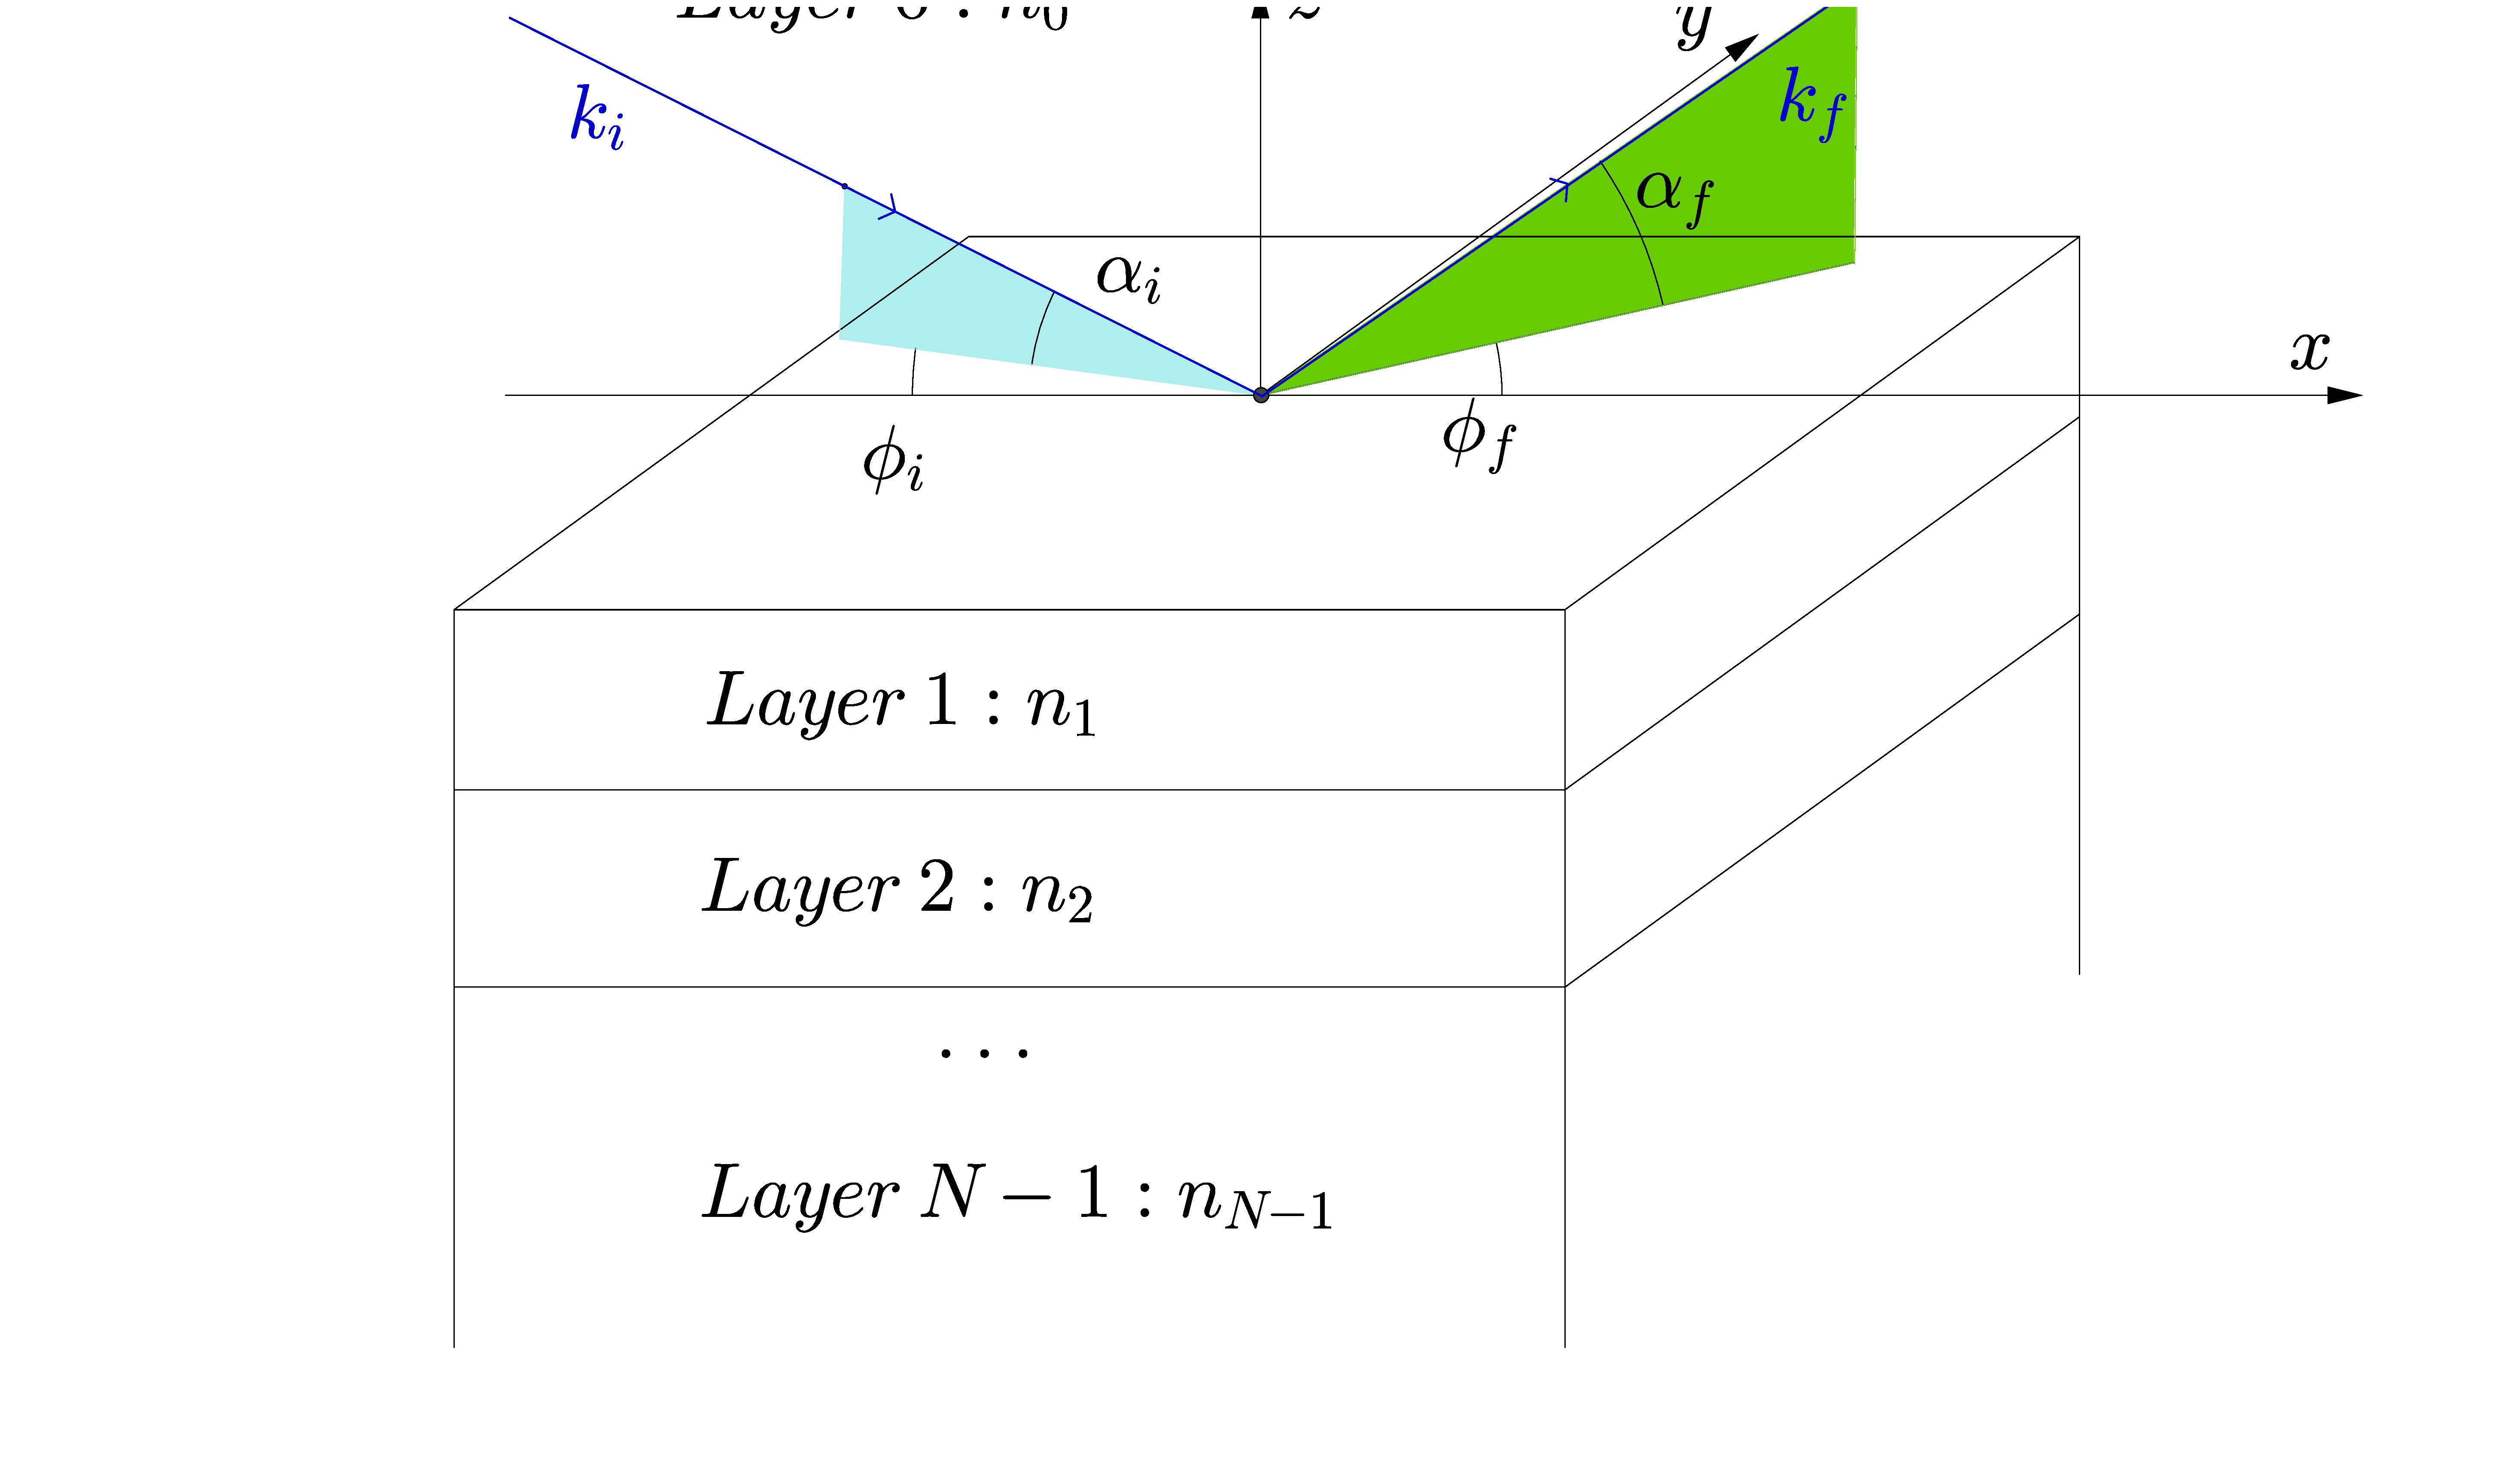
\includegraphics[clip=, width=120mm]{Figures/multilayer3d3.eps}
  \caption[Representation of the scattering geometry.]{Representation of the scattering geometry. $n_j$ is
    the refractive index of layer $j$ and $\alpha_i$ and $\phi_i$ are the incident
    angle of the wave propagating. $\alpha_f$ is the exit angle with respect to the sample's surface and
$\phi_f$ is the scattering angle with respect to the scattering
plane. }
  \label{fig:multil3d}
\end{figure}

\noindent The input beam is assumed to be monochromatic without any
spatial divergence.\\ %\textbf{polarization term?}

\subsection{Units}
By default the angles are expressed in radians and the lengths are given in
nanometers.  But it is possible to use other units by
specifying them right after the value of the corresponding
parameter like, for example, \Code{20.0*micrometer}.


\subsection{Programs}

The examples presented in the next paragraphs are written in Python. For tutorials about this
   programming language, the users are referred to \cite{Pythonref}.

%\noindent Note about the version of C++ and Python to run the examples.\\
%\noindent Where can the following examples be found?\\
%\noindent What is the command to run the examples?

%%%%%%%%%%%%%%%%%%%%%%%%%%%%%%%%%%%%%%%%%%%%
\mysection{Example 1}{Example 1: Two types of islands on top of
  substrate. No interference function} \SecLabel{Example1Python}
% \sectionmark{Example 1}

In this example, we simulate the scattering from a mixture of
cylindrical and prismatic nanoparticles without any interference
between them. These particles are placed in air, on top
of a substrate.\\ We are going to go through each step of the
simulation. The Python script specific to each stage will be given at
the beginning of the description. But for the sake of completeness the full code is given
at the end of this section (Listing~\ref{script_ex1}). \\

\noindent We start by importing different functions from external
modules (line~\ref{import_lib}), for example NumPy, which
is a fundamental package for scientific computing with Python \cite{NumPyURL}.  In particular, line~\ref{import_end}
imports the features of \BornAgain\ software.\\

\begin{lstlisting}[language=python, style=eclipseboxed,name=ex1,nolol]
import sys, os, numpy @\label{import_lib}@

from libBornAgainCore import * @\label{import_end}@
\end{lstlisting}


 %%%%%%%%%%%%%  
\myparagraph{\underline{First step:} Defining materials} 
 

\begin{lstlisting}[language=python, style=eclipseboxed,name=ex1,nolol]
def RunSimulation(): @\label{def_function}@
    #  defining materials @\label{material1}@
    mAmbience = MaterialManager.getHomogeneousMaterial("Air", 0.0, 0.0)  @\label{material2}@
    mSubstrate = MaterialManager.getHomogeneousMaterial("Substrate",
    6e-6, 2e-8) @\label{material3}@
    mParticle = MaterialManager.getHomogeneousMaterial("Particle", 6e-4,
  2e-8 ) @\label{materialparticle}@
\end{lstlisting}

\noindent Line~\ref{def_function} marks the beginning of the
function to define and run the simulation. 

\noindent Lines~\ref{material2}, \ref{material3} and \ref{materialparticle} define different
materials using function \Code{getHomogeneousMaterial} from class
\Code{MaterialManager}. The general syntax is the following 

\begin{lstlisting}[language=python, style=eclipse,numbers=none]
<material_name> = MaterialManager.getHomogeneousMaterial("name", delta, beta)
\end{lstlisting}

\noindent where \Code{name} is the name of the
material associated with its complex refractive index
n=1-\Code{delta} +i \Code{beta}. \Code{<material\_name>} is later used when
referring to this particular material. The three defined materials in this example are \Code{Air} with a refractive
index of 1 (\Code{delta = beta =0}), a \Code{Substrate} associated with a complex refractive index
equal to $1-6\times 10^{-6} +i2\times 10^{-8} $, and the material of particles, whose refractive index is \Code{n}$=1-6\times 10^{-4}+i2\times 10^{-8}$.\\\\

%\noindent \underline{Remark:} there is no condition on the choice of \Code{name}. 
 %%%%%%%%%%%%% 
\myparagraph{\underline{Second step:} Defining the particles} 

\begin{lstlisting}[language=python,style=eclipseboxed,name=ex1,nolol]
    # collection of particles @\label{particles1}@
    cylinder_ff = FormFactorCylinder(5*nanometer, 5*nanometer) @\label{particlescyl1}@
    cylinder = Particle(mParticle, cylinder_ff) @\label{particlescyl2}@
    prism_ff = FormFactorPrism3(5*nanometer, 5*nanometer) @\label{particlesprism1}@
    prism = Particle(mParticle, prism_ff) @\label{particlesprism2}@
\end{lstlisting}

 \noindent We implement two different shapes of particles: cylinders and
 prisms (\textit{i.e.} elongated particles with a constant equilateral triangular cross section).\\ All particles implemented in \BornAgain\ are defined by their
 form factors, their sizes and the material
  they are made of. Here, for the
  cylindrical particle, we input its radius and height.  For the prism, 
  the possible inputs are the length of one side of its equilateral triangular
  base and its height.\\

%\noindent In line~\ref{complx_ref_index}, we define the complex refractive index
%associated with both particle shapes: \Code{n}$=1-6\times 10^{-4}+i2\times 10^{-8}$.\\
  
\noindent In order to define a particle, we proceed in two steps. For example for
the cylindrical particle, we first specify the form factor of a cylinder with 
its radius and height, both equal to 5 nanometers in this particular
case (see line~\ref{particlescyl1}). Then we associate this shape with
the constituting material as in line~\ref{particlescyl2}.\\

\noindent The same procedure has been applied for the prism in lines~\ref{particlesprism1} and \ref{particlesprism2} respectively.
 %%%%%%%%%%%%% 
\myparagraph{\underline{Third step:} Characterizing the layers and assembling the sample} 

\noindent \textbf{Particle decoration} \\
  

\begin{lstlisting}[language=python, style=eclipseboxed, name=ex1,nolol]
    particle_decoration = ParticleDecoration()  @\label{particlesdecor1}@
    particle_decoration.addParticle(cylinder, 0.0, 0.5)  @\label{particlesdecor2}@
    particle_decoration.addParticle(prism, 0.0, 0.5)@\label{particlesdecor3}@
    interference = InterferenceFunctionNone()  @\label{particlesnointerf}@
    particle_decoration.addInterferenceFunction(interference)  @\label{particlesinterf}@
\end{lstlisting}

\noindent The object which holds the information about the positions and densities of particles
in our sample is called \Code{ParticleDecoration}
(line~\ref{particlesdecor1}). We use the associated function \Code{addParticle}
for each particle shape (lines~\ref{particlesdecor2}, \ref{particlesdecor3}). Its general
syntax is 

\begin{lstlisting}[language=python, style=eclipse,numbers=none]
addParticle(<particle_name>, depth, abundance) 
\end{lstlisting}

\noindent  where \Code{<particle\_name>} is the name used to define the particles
(lines~\ref{particlescyl2} and \ref{particlesprism2}), \Code{depth}
(default value =0)
is the vertical position, expressed in nanometers, of the particles in a given layer (the
association with a particular layer will be done during the next step) and
\Code{abundance} is the proportion of this type of particles, 
normalized to the total number of particles. Here we have 50\% of cylinders
and 50\% of prisms. \\ 

\ImportantPoint{Remark:}{Depth of particles\\
The vertical positions of particles in a layer are given in relative
coordinates. For the top layer, the bottom corresponds to
\Code{depth}=0 and negative values would correspond to particles
floating above layer 1 since the vertical axis, shown in \reffig{multil3d} is pointing upwards. But for all the other layers, it is the top of the
layer which corresponds to \Code{depth}=0.}\\


\noindent Finally lines~\ref{particlesnointerf} and
\ref{particlesinterf} specify that there is \textbf{no coherent interference} between
the waves scattered by these particles. The intensity is calculated by
the incoherent sum of the scattered waves: $\langle |F_n|^2\rangle$,
where $F_n$ is the form factor associated with the particle of type $n$.  The way these waves
interfere imposes the horizontal distribution of
the particles as
the interference reflects the long or short-range order of the
particles distribution (\textbf{see Theory}). On the contrary, the vertical position is
imposed when we add the particles in a given layer by parameter \Code{depth}, as shown in lines~\ref{particlesdecor2} and \ref{particlesdecor3}. \\

\noindent \textbf{Multilayer}\\
  
\begin{lstlisting}[language=python, style=eclipseboxed,name=ex1,nolol]
    # air layer with particles and substrate form multi layer  @\label{sampleassembling}@
    air_layer = Layer(mAmbience)  @\label{airlayer}@
    air_layer.setDecoration(particle_decoration)  @\label{airlayerdecorator}@
    substrate_layer = Layer(mSubstrate, 0)  @\label{substratelayer}@
    multi_layer = MultiLayer()  @\label{multilayercanvas}@
    multi_layer.addLayer(air_layer)  @\label{layerairdecor}@
    multi_layer.addLayer(substrate_layer)  @\label{layersubstrate}@
\end{lstlisting}

\noindent We now have to configure our sample. For this first example,
the particles, \textit{i.e.} cylinders and prisms, are on top of a substrate in an
air layer. \textbf{The order in which we define these layers is important: we
start from the top layer down to the bottom one}.\\

\noindent Let us start with the air layer. It contains the particles. In
line~\ref{airlayer}, we use the previously defined \Code{mAmbience}
(="air" material) (line~\ref{material2}). The command written in line~\ref{airlayerdecorator} shows that this layer is decorated by adding the
particles using the function \Code{particle\_decoration} defined in
lines~\ref{particlesdecor1}-\ref{particlesinterf}. The substrate layer
only contains the substrate material (line~\ref{substratelayer}).\\%Note that the
%\Code{depth} is referenced to the bottom of the top layer (negative
%values would correspond to particles floating above layer 1 as
%the vertical axis is pointing upwards). 
 
\noindent There are different possible syntaxes to define a layer. As shown in
lines~\ref{airlayer} and \ref{substratelayer}, we can use
\Code{Layer(<material\_name>,thickness)} or
\Code{Layer(<material\_name>)}. The second case corresponds
to the default value of the \Code{thickness}, equal to 0. The \Code{thickness} is
expressed in  nanometers. \\

\noindent Our two layers are now fully characterized. The sample is assembled using
\Code{MultiLayer()} constructor (line~\ref{multilayercanvas}): we start with the air layer decorated
with the particles (line~\ref{layerairdecor}), which is the layer at
the top and end with the bottom layer, which is the
substrate (line~\ref{layersubstrate}).
 %%%%%%%%%%%%% 
\myparagraph{\underline{Fourth step:} Characterizing the input beam and
output detector and running the simulation} 


\begin{lstlisting}[language=python, style=eclipseboxed,name=ex1,nolol]
    # run simulation  @\label{run1}@
    simulation = Simulation()  @\label{run2}@
    simulation.setDetectorParameters(100,-1.0*degree, 1.0*degree, 
                                100, 0.0*degree, 2.0*degree, True)  @\label{rundetector}@
    simulation.setBeamParameters(1.0*angstrom, 0.2*degree, 0.0*degree)  @\label{runbeam}@
    simulation.setSample(multi_layer)  @\label{runsample}@
    simulation.runSimulation()  @\label{runsimul}@
\end{lstlisting}


\noindent The first stage is to define the \Code{Simulation()} object (line~\ref{run2}). Then we define the detector (line~\ref{rundetector}) and beam
parameters (line~\ref{runbeam}), which are associated with the
sample previously defined (line~\ref{runsample}). Finally we run
the simulation (line~\ref{runsimul}). Those functions are part of the Simulation
class.  The
different incident and exit angles are
shown in \reffig{multil3d}. \\

\noindent The detector parameters are set using ranges of angles via
the function:\\

\noindent \Code{setDetectorParameters(n\_phi, phi\_f\_min,
  phi\_f\_max,\\ \phantom{setDetectorParameters(}n\_alpha, alpha\_f\_min, alpha\_f\_max, isgisaxs\_style=false)}, \\

\noindent where \Code{n\_phi=100} is the number of iterations for $\phi_f$,\\ \Code{phi\_f\_min=-1.0*degree} and \Code{phi\_f\_max=1.0*degree}
are the minimum and maximum values respectively of $\phi_f$, \\ \Code{n\_alpha=100} is
the number of iterations for $\alpha_f$,\\ \Code{alpha\_f\_min=0.0*degree} and \Code{alpha\_f\_max=2.0*degree} 
are the minimum and maximum values respectively of
$\alpha_f$. \\
\Code{isgisaxs\_style=True} (default value = \Code{False}) is a boolean
used to characterise the structure of the output data. If
\Code{isgisaxs\_style=True}, the output data is binned at constant
values of the sine of the output angles, $\alpha_f$ and $\phi_f$, otherwise it is binned
at constant values of these two angles.\\


\noindent For the beam the function to use is
\Code{setBeamParameters(lambda, alpha\_i, phi\_i)}, where\\
\Code{lambda=1.0*angstrom} is the incident beam wavelength,
\Code{alpha\_i=0.2*degree} is the incident
grazing angle on the surface of the sample,
\Code{phi\_i=0.0*degree} is the in-plane
direction of the incident beam (measured with respect to the
$x$-axis).\\ 

\noindent \underline{Remark}: Note that, except for
\Code{isgisaxs\_style}, there are no default values implemented for the
parameters of the beam and detector.\\

\noindent Line~\ref{runsimul} shows the command to run the simulation using the
previously defined setup.
%%%%%%%%%%%%%
\myparagraph{\underline{Fifth step:} Saving the data} 


\begin{lstlisting}[language=python, style=eclipseboxed,name=ex1,nolol]
    # retrieving intensity data
    return GetOutputData(simulation) @\label{outputdata}@
\end{lstlisting}


\noindent In line~\ref{outputdata} we obtain the simulated intensity
as a function of outgoing angles $\alpha_f$ and $\phi_f$ for further
uses (plots, fits,\ldots) as a NumPy array containing
\Code{n\_phi}$\times$\Code{n\_alpha}
datapoints. Some options are provided by \BornAgain. For example, \reffig{output_ex1} shows the two-dimensional
contourplot of the intensity as a function of $\alpha_f$ and
$\phi_f$. 

\begin{figure}[h]
  \begin{center}
   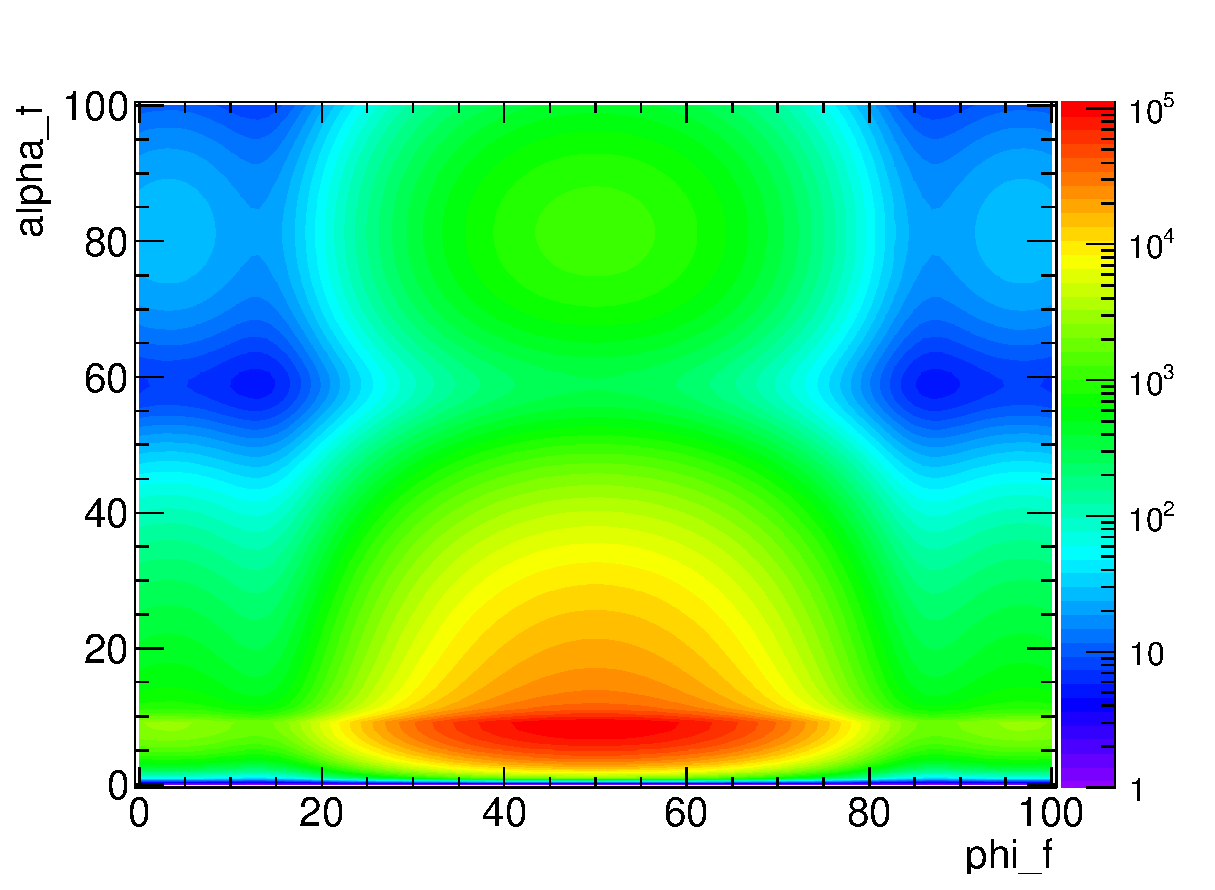
\includegraphics[clip=true, width=120mm]{Figures/Manual_ex1.eps}
  \end{center}
  \caption[Example 1: Simulated grazing-incidence small-angle X-ray scattering from a mixture of
cylindrical and prismatic nanoparticles without any interference, deposited on top
of a substrate]{Figure of example 1: Simulated grazing-incidence small-angle X-ray scattering from a mixture of
cylindrical and prismatic nanoparticles without any interference, deposited on top
of a substrate. The input beam is characterized by a wavelength
$\lambda$ of 1~\AA\ and incident angles $\alpha_i=0.2^{\circ}$, $\phi_i=0^{\circ}$. The
cylinders have a radius and a height both equal to 5~nm, the prisms
are characterized by a side length equal to 5~nm and they are also 5~nm high. The
material of the particles has a refractive index of $1-6\times 10^{-4}+i2\times 10^{-8}$. For the substrate
it is equal to $1-6\times 10^{-6} +i2\times 10^{-8} $. The colorscale
is associated with the output intensity in arbitrary units. }
\label{fig:output_ex1}
\end{figure}

\newpage
\begin{lstlisting}[caption={Python script of example 1},
  label=script_ex1,captionpos=b,escapeinside={@}{@} ,language=python,style=eclipse, numbers= none,frame = leftline ,
      framerule = 2mm ,
      rulecolor = \color{lightgrey},
      breaklines = true]
import sys, os, numpy 

sys.path.append(os.path.abspath(os.path.join(os.path.split(__file__)[0],'..', '..', '..', 'lib')))

from libBornAgainCore import * 

def RunSimulation():
    #  defining materials 
    mAmbience = MaterialManager.getHomogeneousMaterial("Air", 0.0, 0.0 ) 
    mSubstrate = MaterialManager.getHomogeneousMaterial("Substrate",
    6e-6, 2e-8) 
    mParticle = MaterialManager.getHomogeneousMaterial("Particle", 6e-4, 2e-8 )
    # collection of particles 
    cylinder_ff = FormFactorCylinder(5*nanometer, 5*nanometer) 
    cylinder = Particle(mParticle, cylinder_ff) 
    prism_ff = FormFactorPrism3(5*nanometer, 5*nanometer) 
    prism = Particle(mParticle, prism_ff) 
    particle_decoration = ParticleDecoration()  
    particle_decoration.addParticle(cylinder, 0.0, 0.5)  
    particle_decoration.addParticle(prism, 0.0, 0.5)  
    interference = InterferenceFunctionNone()  
    particle_decoration.addInterferenceFunction(interference)  
    # air layer with particles and substrate form multi layer 
    air_layer = Layer(mAmbience)  
    air_layer.setDecoration(particle_decoration)
    substrate_layer = Layer(mSubstrate, 0) 
    multi_layer = MultiLayer()  
    multi_layer.addLayer(air_layer) 
    multi_layer.addLayer(substrate_layer) 

    # build and run simulation  
    simulation = Simulation()  
    simulation.setDetectorParameters(100,-1.0*degree, 1.0*degree, 
                                    100, 0.0*degree, 2.0*degree, True) 
    simulation.setBeamParameters(1.0*angstrom, 0.2*degree, 0.0*degree) 
    simulation.setSample(multi_layer) 
    simulation.runSimulation()  

    # retrieving intensity data
     return GetOutputData(simulation)
\end{lstlisting}

% \newpage
% \subsection{Hello, minted}
% 
% \begin{minted}[linenos=true, frame=single]{python}
% mAmbience = MaterialManager.getHomogeneousMaterial("Air", 1.0, 0.0 )
% mSubstrate = MaterialManager.getHomogeneousMaterial("Substrate", 1.0-6e-6, 2e-8 )
% n_particle = complex(1.0-6e-4, 2e-8)
% cylinder_ff = FormFactorCylinder(5*nanometer, 5*nanometer)
% cylinder = Particle(n_particle, cylinder_ff)
% prism_ff = FormFactorPrism3(5*nanometer, 5*nanometer)
% prism = Particle(n_particle, prism_ff)
% particle_decoration = ParticleDecoration()
% particle_decoration.addParticle(cylinder, 0.0, 0.5)
% particle_decoration.addParticle(prism, 0.0, 0.5)
% interference = InterferenceFunctionNone()
% particle_decoration.addInterferenceFunction(interference)
% # air layer with particles and substrate form multi layer
% air_layer = Layer(mAmbience)
% air_layer_decorator = LayerDecorator(air_layer, particle_decoration)
% substrate_layer = Layer(mSubstrate, 0)
% multi_layer = MultiLayer()
% multi_layer.addLayer(air_layer_decorator)
% multi_layer.addLayer(substrate_layer)
% 
% # build and run experiment
% simulation = Simulation()
% simulation.setDetectorParameters(100,-1.0*degree, 1.0*degree, 100, 0.0*degree, 2.0*degree, True)
% simulation.setBeamParameters(1.0*angstrom, -0.2*degree, 0.0*degree)
% simulation.setSample(multi_layer)
% simulation.runSimulation()
% \end{minted}

\section{Example 2}





\end{document}

